\subsection{Descripción del problema.}

\vspace*{0.3cm}

Luego del éxito rotundo del último ataque contra los zombies producido por nuestro anterior algoritmo, la humanidad ve un rayo de esperanza.

En una de las últimas ciudades tomadas por la amenaza Z, se encuentra un científico que afirma haber encontrado la cura contra el zombieismo, rodeado por una cuadrilla de soldados del más alto nivel. Nuestro noble objetivo es, entonces, proveer del camino más seguro (el que genere menos perdidas humanas) al científico y sus soldados de manera tal que logren llegar desde donde están, hasta el bunker militar que se encuentra en esa ciudad. Para esto, se conocen los siguientes datos:

\begin{itemize}
	\item La ciudad en cuestión tiene la forma clásica de grilla rectangular, compuesta por $n$ calles paralelas en forma horizontal, $m$ calles paralelas en forma vertical dando así una grilla de manzanas cuadradas. Los numeros $n$ y $m$ son conocidos.
	\item Se conoce la ubicación del científico y del bunker.
	\item Se conoce la cantidad de soldados que el científico tiene a su disposición.
	\item Si todos los soldados perecen, el científico no tiene posibilidad de sobrevivir por sí mismo (o sea, no podemos llegar al bunker con 0 soldados).
	\item Se sabe la cantidad de zombies ubicados en cada calle.
	\item Si bien nuestros soldados tienen un alto nivel de combate, el enfrentamiento que tuvieron en el último ataque contra los zombies, acabaron con todas sus municiones por lo cual solo tienen sus cuchillos de combate. Esto incide entonces, en que el grupo sólo pasará por una calle sin sufrir pérdidas si hay hasta un soldado por zombie, al menos, y en caso contrario, perderá la diferencia entre la cantidad de soldados, y la cantidad de zombies. En otras palabras, sea $z$ la cantidad de zombies de una calle, y $s$ la cantidad de soldados de que tiene la cuadrilla al momento de pasar por esa calle, si $s \geq z$ entonces la cuadrilla pasa sin perdidas; en caso contrario la cuadrilla pierde $z - s$ soldados.
	\item Puede no existir un camino que asegure la supervivencia del científico.
	\item La complejidad del algoritmo pedido es de $\mathcal{O}(s \cdot n \cdot m)$.
	\item La salida de este algoritmo deberá mostrar la cantidad de soldados que llegan vivos al bunker, seguido de una línea por cada esquina del camino recorrido, representada por dos enteros indicando la calle horizontal y la vertical que conforman dicha intersección.  En caso de no existir solución, se mostrará el valor 0. 
\end{itemize}

Ejemplo: 

Supongamos una ciudad como muestra la Figura \ref{fig:ejzombie}, donde los números indican la cantidad de zombies en cada cuadra. Consideremos que la cantidad de soldados al comenzar es 10.
%
%\begin{figure}[htb]
%	\begin{center}
%    		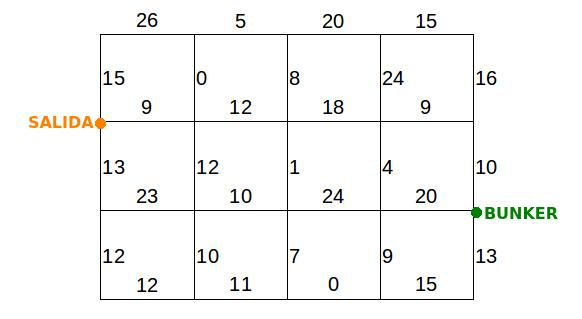
\includegraphics[scale=0.5]{imagenes/ejemplozombie.jpeg}
%	\end{center}
%	\caption{Ejemplo de ciudad para Zombieland II}\label{fig:ejzombie}
%\end{figure}
%
La solución para este ejemplo permite llegar al búnker sin perder ningún soldado, siendo el recorrido el indicado en la Figura \ref{fig:ejzombieres}.
%
%\begin{figure}[htb]
%	\begin{center}
%    		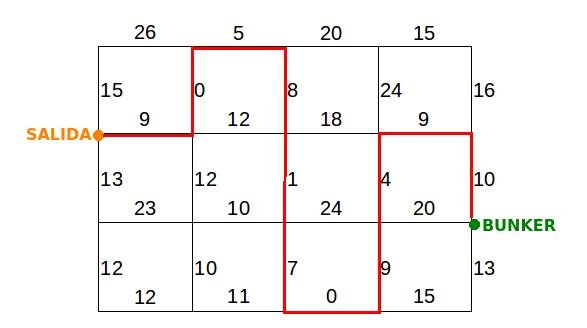
\includegraphics[scale=0.5]{imagenes/ejemplozombieres.jpeg}
%	\end{center}
%	\caption{Solución para el problema de la Figura \ref{fig:ejzombie}}\label{fig:ejzombieres}
%\end{figure}

\begin{figure}[!htb]
\minipage{0.5\textwidth}
  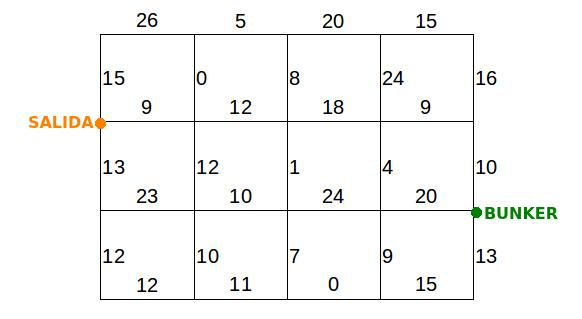
\includegraphics[scale=0.5]{imagenes/ejemplozombie.jpeg}
  \caption{Ejemplo de ciudad para Zombieland II}\label{fig:ejzombie}
\endminipage
\minipage{0.5\textwidth}
  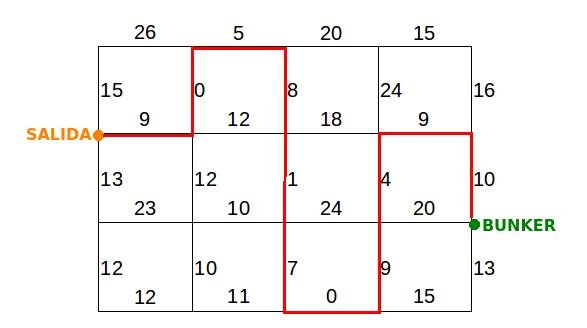
\includegraphics[scale=0.5]{imagenes/ejemplozombieres.jpeg}
  \caption{Solución para el problema de la Figura \ref{fig:ejzombie}}\label{fig:ejzombieres}
\endminipage
\end{figure}


\vspace*{0.6cm}

%\newpage
\subsection{Desarrollo de la idea y correctitud.}

\vspace*{0.3cm}

Debemos recorrer la ciudad en busca de un camino que permita llegar al búnker con la mayor cantidad de soldados vivos.  Sin embargo, probar todos los posibles caminos tomaría más tiempo del que disponemos en un ataque zombie.  Por lo tanto, hemos decidido buscar dicho camino de la siguiente manera:

Utilizando {\it backtraking}, trataremos de encontrar las rutas que salen desde la posición de origen, de manera que ningún soldado muera.  Cada cuadra visitada será marcada para que ningún otro camino intente pasar por ahí, y así no tendremos caminos redundantes (es decir, no consideraremos distintos caminos que permitan llegar a una misma esquina con la misma cantidad de soldados vivos), y para cada esquina alcanzada se guardará la esquina anterior de ese camino y la cantidad de soldados vivos hasta ese momento.  Si en algún momento se llega a una esquina con alguna cuadra incidente por la cual no se puede avanzar sin pérdidas, vamos a señalizarla (en breve explicaremos para qué).

Si por alguno de estos caminos se llega al búnker, entonces habremos encontrado una solución óptima.  Si ninguna de las rutas encontradas es solución, entonces deberemos animarnos a perder soldados.  Para ello, primero vamos a arriesgar sólo un soldado, es decir, si teníamos $s$ soldados iniciales, intentaremos llegar al búnker con $s-1$ soldados vivos. Entonces, retomaremos los caminos marcados anteriormente, a partir de las esquinas desde las que no podíamos avanzar sin pérdidas (reanudando cada una en el orden en el que fueron marcadas).  Desde ahí, avanzaremos armando los caminos que no nos produzcan más de una baja, y lo haremos de la misma manera que explicamos arriba: guardando la esquina antecesora y la cantidad de soldados vivos en cada esquina atravesada, y sin considerar caminos redundantes. Si al intentar retomar el camino desde una esquina marcada anteriormente, una de las cuadras incidentes produce más de una baja en los soldados, entonces la esquina seguirá estando marcada para alguna etapa posterior.

Nuevamente, si alguno de estos caminos llega al búnker, será la solución.  Caso contrario repetiremos el procedimiento intentando llegar con $s-2$ soldados vivos. De forma sucesiva, nos animaremos a perder cada vez un soldado más, y el primer camino encontrado que llegue al búnker será retornado. 

Puede suceder que mediante una ruta se llegue a una esquina por la que ya pasó otro camino. Dado que las esquinas marcadas las vamos retomando en el orden en el que fueron marcadas, y que en cada esquina que se retoma se puede perder igual o más número de soldados, entonces el camino que pasó primero por una esquina lo hizo con igual o mayor cantidad de soldados vivos que el segundo.  Como no queremos considerar caminos redundantes, si ambas rutas llegan con la misma cantidad de soldados vivos, descartaremos uno de ellos. Y si el primer camino tiene más soldados vivos que el segundo en ese momento, la continuación de ellos podría, o bien, producir pérdidas en los soldados del segundo camino y no en los del primero, o bien producir pérdidas en ambos, pero con menor impacto en el primero que en el segundo. Por lo tanto, resulta conveniente considerar el camino con mayor cantidad de soldados vivos, y por este motivo se decidió que al suceder un cruce de caminos como el expuesto, sólo se tendrá en cuenta aquél que haya ocurrido primero. De esta manera, estamos asegurando que la solución tiene la mayor cantidad de soldados vivos al final. 

En caso de llegar al punto de tener un sólo soldado vivo y no encontrar un camino que llegue al búnker, significa que no hay solución.

Una vez que se llega al búnker, se debe ``rearmar'' el camino correcto.  Por lo explicado anteriormente, cada esquina será atravesada por a lo sumo 1 camino, y por lo tanto tendrá a lo sumo 1 esquina antecesora. Entonces basta con consultar consecutivamente ese dato desde la posición del búnker hasta llegar al punto de partida.

Las Figuras \ref{fig:ejzombie0}, \ref{fig:ejzombie1}, \ref{fig:ejzombie2}, \ref{fig:ejzombie3} y \ref{fig:ejzombie4} muestran la forma de operar del algoritmo descrito. Notar que luego de encontrar los posibles caminos perdiendo hasta 1 soldado (\ref{fig:ejzombie2}), no existe ningún camino posible que nos permita avanzar con a lo sumo 2 pérdidas, y por eso se prosigue por un camino que soporte hasta 3 pérdidas (\ref{fig:ejzombie3}).

\begin{figure}[!htb]
\minipage{0.5\textwidth}
  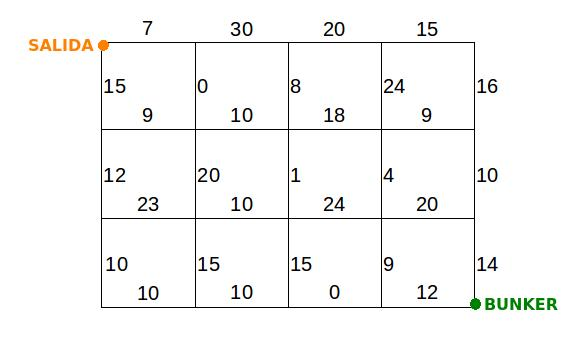
\includegraphics[scale=0.5]{imagenes/ejzombie0.jpeg}
  \caption{Ejemplo de ciudad - 11 soldados iniciales}\label{fig:ejzombie0}
\endminipage
\minipage{0.5\textwidth}
  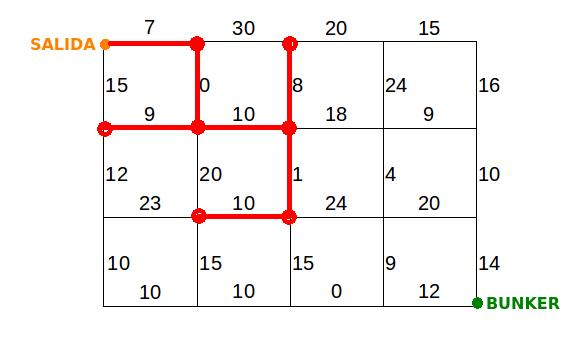
\includegraphics[scale=0.5]{imagenes/ejzombie1.jpeg}
  \caption{Caminos para la Figura \ref{fig:ejzombie0} sin pérdidas}\label{fig:ejzombie1}
\endminipage\\
\minipage{0.5\textwidth}
  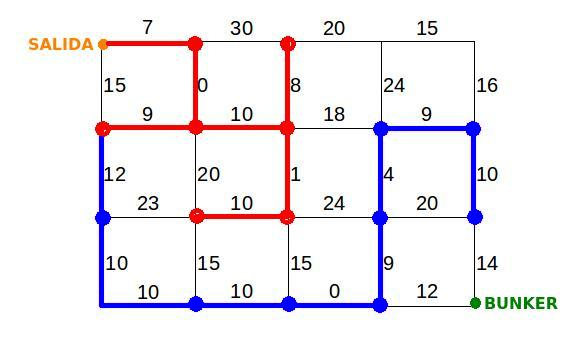
\includegraphics[scale=0.5]{imagenes/ejzombie2.jpeg}
  \caption{Continuación de Figura \ref{fig:ejzombie1} con 1 pérdida}\label{fig:ejzombie2}
\endminipage
\minipage{0.5\textwidth}
  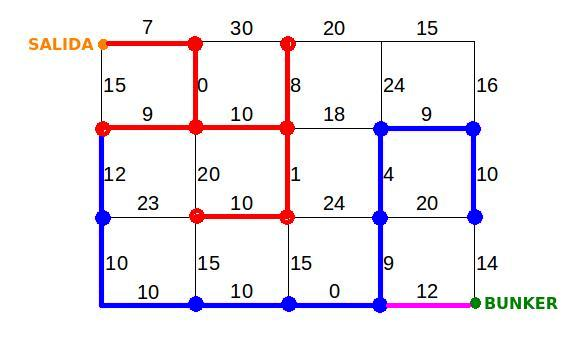
\includegraphics[scale=0.5]{imagenes/ejzombie3.jpeg}
  \caption{Continuación de Figura \ref{fig:ejzombie2} con 3 pérdidas}\label{fig:ejzombie3}
\endminipage\\
\minipage{0.5\textwidth}
  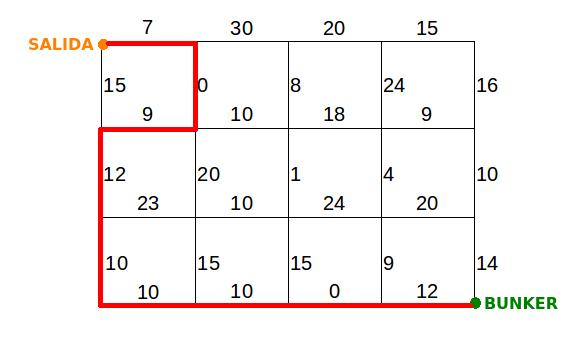
\includegraphics[scale=0.5]{imagenes/ejzombie4.jpeg}
  \caption{Solución para la Figura \ref{fig:ejzombie0}}\label{fig:ejzombie4}
\endminipage
\end{figure}


\vspace*{0.6cm}

%\newpage
%\subsection{Justificación de la resolución y demostración de correctitud.}

%\vspace*{0.3cm}



%\vspace*{0.6cm}

%\newpage
\subsection{Análisis de complejidad.}

\vspace*{0.3cm}

Llamemos $n$ la cantidad de calles horizontales y $m$ la cantidad de calles verticales.  Tomando $1 \leq i \leq n$ y $1 \leq j \leq m$, la esquina $(i,j)$ será la esquina formada por la intersección de las calles $i$ y $j$.  Para cada esquina definimos los siguientes atributos:

\begin{itemize}
	\item {\bf Arriba}: cuadra a atravesar para moverse a la esquina $(i-1,j)$. Se considerará inválido cuando $i = 1$.
	\item {\bf Abajo}: cuadra a atravesar para moverse a la esquina $(i+1,j)$. Se considerará inválido cuando $i = n$.
	\item {\bf Izquierda}: cuadra a atravesar para moverse a la esquina $(i,j-1)$. Se considerará inválido cuando $j = 1$.
	\item {\bf Derecha}: cuadra a atravesar para moverse a la esquina $(i,j+1)$. Se considerará inválido cuando $j = m$.
	\item {\bf Origen}: nombre de la esquina antecesora, en caso de existir.  Si la esquina aún no ha sido visitada, permanecerá vacío.
	\item {\bf Parcial}: cantidad de soldados vivos al llegar a la esquina desde {\bf Origen}. Si la esquina aún no ha sido visitada, permanecerá vacío.
\end{itemize}

\begin{figure}[!ht]
\begin{codebox}
\Procname{$\proc{Zombieland}(soldados,inicio,bunker)$}
\li $tope \leftarrow soldados$
\li $marcados \leftarrow$ lista vacía de esquinas
\li $marcados \leftarrow$ agregar atrás $inicio$
\li $res \leftarrow$ false
\li \While $tope > 0$ y $\neg res$
\li		\Do \While $marcados$ siga teniendo elementos de la etapa anterior
\li				\Do
					$esquina \leftarrow$ desencolar primer elemento de $marcados$
\li					$res \leftarrow res$ + {\sc Recorridos}($marcados,soldados,esquina,bunker,tope$)
				\End
\li			decrementar $tope$
		\End
\li	\If $\neg res$
\li		\Do $soldados \leftarrow 0$ \End
\li		\Else 
\li			\Do $soldados \leftarrow tope + 1$
			\End
		\End
\end{codebox} 
\caption{Pseudocódigo de Zombieland II}\label{code:zombieland}
\end{figure}
%\FloatBarrier


\begin{figure}[!ht]
\begin{codebox}
\Procname{Bool $\proc{Recorridos}(marcados,soldados,esquina,bunker,tope)$}
\li $res \leftarrow$ false
\li \If $esquina == bunker$
\li 		\Do \Return true
		\End
\li 	\If se puede ir hacia $esquina.derecha$
\li 		\Do \If se mueren soldados cumpliendo $tope$
\li				\Do 
					$soldados \leftarrow$ actualizar
				\End
\li			$siguiente \leftarrow$ esquina a la que se llega
\li			inhabilitar $esquina.derecha$ y $siguiente.izquierda$
\li			\If $siguiente.origen$ y $siguiente.parcial$ están vacíos
\li				\Do
					$siguiente.origen \leftarrow esquina$
\li					$siguiente.parcial \leftarrow soldados$
				\End
\li			$res \leftarrow res$ + {\sc Recorridos}($marcados,soldados,siguiente,bunker,tope$)
\li			\If $res$ 
\li				\Do \Return $res$
				\End
		\End
\li 	\If se puede ir hacia $esquina.abajo$
\li 		\Do \If se mueren soldados cumpliendo $tope$
\li				\Do 
					$soldados \leftarrow$ actualizar
				\End
\li			$siguiente \leftarrow$ esquina a la que se llega
\li			inhabilitar $esquina.abajo$ y $siguiente.arriba$
\li			\If $siguiente.origen$ y $siguiente.parcial$ están vacíos
\li				\Do
					$siguiente.origen \leftarrow esquina$
\li					$siguiente.parcial \leftarrow soldados$
				\End
\li			$res \leftarrow res$ + {\sc Recorridos}($marcados,soldados,siguiente,bunker,tope$)
\li			\If $res$ 
\li				\Do \Return $res$
				\End
		\End
\li 	\If se puede ir hacia $esquina.arriba$
\li 		\Do \If se mueren soldados cumpliendo $tope$
\li				\Do 
					$soldados \leftarrow$ actualizar
				\End
\li			$siguiente \leftarrow$ esquina a la que se llega
\li			inhabilitar $esquina.arriba$ y $siguiente.abajo$
\li			\If $siguiente.origen$ y $siguiente.parcial$ están vacíos
\li				\Do
					$siguiente.origen \leftarrow esquina$
\li					$siguiente.parcial \leftarrow soldados$
				\End
\li			$res \leftarrow res$ + {\sc Recorridos}($marcados,soldados,siguiente,bunker,tope$)
\li			\If $res$ 
\li				\Do \Return $res$
				\End
		\End		
\li 	\If se puede ir hacia $esquina.izquierda$
\li 		\Do \If se mueren soldados cumpliendo $tope$
\li				\Do 
					$soldados \leftarrow$ actualizar
				\End
\li			$siguiente \leftarrow$ esquina a la que se llega
\li			inhabilitar $esquina.izquierda$ y $siguiente.derecha$
\li			\If $siguiente.origen$ y $siguiente.parcial$ están vacíos
\li				\Do
					$siguiente.origen \leftarrow esquina$
\li					$siguiente.parcial \leftarrow soldados$
				\End
\li			$res \leftarrow res$ + {\sc Recorridos}($marcados,soldados,siguiente,bunker,tope$)
\li			\If $res$ 
\li				\Do \Return $res$
				\End
		\End
\li \If no se pudo avanzar en alguno de los sentidos por exceso de zombies
\li 		\Do 	$marcados \leftarrow$ agregar al final $esquina$
		\End
\li \Return false
\end{codebox} 
\caption{Pseudocódigo para la búsqueda de recorridos en la ciudad}\label{code:zombieland.rec}
\end{figure}
\FloatBarrier

\vspace*{0.6cm}

%\newpage
\subsection{Experimentación y gráficos.}


\subsubsection{Test 1}

\vspace*{0.3cm}


\vspace*{0.6cm}

%\newpage
\subsubsection{Test 2}


\newpage